\subsection{Experimental results}
This section contains experimental results to find the best possible price predicting solution. The results are divided into 5 experiments. The first experiment finds the best combination of input parameters for the network. These input parameters count meteorological, social and seasonal factors we identified in section~\ref{sec:Price}. The next experiment identifies the need for trimming and reasons why it is needed in this particular dataset. The third experiment tests different statistical strategies to incorporate historical prices as a part of the dataset. This includes historical prices, curve behavior analysis, skewness analysis and historical EWMA(Exponentially-Weighted Moving Average). The fourth experiment takes care of the Artificial Neural Network parameters. This includes black-box optimization like pruning of the network and optimization of epochs.

\subsection{Experiment 1: Inputs}
In this section we experimented with the basic input parameters that we identified in section~\ref{sec:Price}. We did a cross comparison of all the inputs and possible combinations (For those that made sense). The Price and the Demand is such a basic measure when you define a price in any markets that they are included in every prediction. We did not make a cross comparison of the Month of Year and the Seasons of Year since they say the same but with different granularity. We did a cross comparison both with and without matrix inputs and with a mix of non-matrix and matrix inputs. This is done to determine whether an input makes better sense on matrix form or just as a simple normalized value. 

Experiment 1 is based on a dataset consisting of the last 3 months averaging to about 2189 hours. We use 200 epochs for each training iteration.

This includes last hours Price (P), The Demand (D), Wind Speed(WS), Temperature(T), The Hourly Time of Day (ToD), The Day of The Week(DoW), The Month of The Year(MoY), The Season of The Year(SoY). The (M) is for Matrix input and states whether the input in the seasonal rows(ToD, WoD, MoY, SoY) are on matrix form or not.

As we saw in the wind production experiments(WPE) section~\ref{sec:windPowerAnalysis} there was a problem regarding the way we conducted tests for the seasonality; specifically for the MoY and the SoY. We only use the last 3 months to train the network and that sort of eliminates the obvious purpose of the MoY and SoY. As we saw in the results for the first experiment in WPE if we include the same month as we are in from last year and reintroduce the purpose of the SoY and MoY it gave us a worse result than leaving it out. To make sure the same thing applies on the price prediction experiments we conducted to runs of all the combinations of inputs. First we ran it with the last 3 months including the same month that we are in from last year and after that we ran the experiment with only the last 3 months.

Table~\ref{table:Top20Prices} shows us the top 20 MAE from the experiment with a training set containing the last 3 months(3Month). We have compared this to the experiment with a training set containing the last 3 months and the same month from last year(4Month). As we see in the table there isn't the biggest deviation between the two datasets. This also shows in \todo{Ref Appendix for both} that the distribution of the MAE over the two datasets are quite similar. From this we can conclude that the effect of using last years month in our dataset does not make a significant difference and can be left out. This raises the question if the MoY and the SoY can be left out as well, since the obvious use for it is eliminated by never having a full month or full season in the training set - that is equal to the one we predict.

First we conducted an experiment containing a training set with a full year (to test the effect of seasonality on a full year) we included the rest of the parameters equal to rank \#1 in table~\ref{table:Top20Prices} and shifted the seasonality. The results can be seen in table~\ref{table:1YearTrain} where we can see the full effect of seasonality over a year. The table clearly shows that the MoY combination is the best of the three. If we compare the results to the results from table~\ref{table:Top20Prices} it shows us that with monthly seasonality the neural network will be able to do the same predictions as the predictions that only have a training set of 3 months. With the possibility of over training in too large datasets(see citation~\cite{1}) and that the neural network takes longer time training on a larger dataset. We can conclude that the smaller dataset of 3 months are better to use than the full year (We will elaborate on this in experiment X)\todo{Saet rigtigt experiment}. Further more we have to test if seasonality being an input parameter makes sense when our dataset is only 3 months big. 

\begin{table}[H]
\centering  % used for centering table
\resizebox{\textwidth}{!}{
\begin{tabular}{|c|c|c|c|c|c|c|c|c|c|c|c|} % centered columns (7 columns)
\hline
P & D & WS & T & ToD & DoW & MoY & SoY & 3Month & 4Month & Rank\\ [0.5ex] % inserts table 
%heading
\hline                  % inserts single horizontal line
 \x    & \x    & \x    & \x    & \x\m  & \x\m  &       & \x\m  & 57.12 & 61.70 & \#1 \\ \hline
 \x    & \x    & \x    & \x    & \x\m  & \x    &       & \x\m  & 58.09 & 68.23 & \#2 \\ \hline
 \x    & \x    & \x    & \x    & \x\m  &       & \x\m  &       & 58.79 & 63.80 & \#3 \\ \hline
 \x    & \x    & \x    &       & \x\m  & \x\m  & \x\m  &       & 60.14 & 67.82 & \#4 \\ \hline
 \x    & \x    & \x    & \x    & \x\m  & \x    &       &       & 62.19 & 74.89 & \#5 \\ \hline
 \x    & \x    & \x    & \x    & \x\m  &       &       & \x\m  & 62.26 & 61.86 & \#6 \\ \hline
 \x    & \x    & \x    & \x    & \x\m  & \x    & \x\m  &       & 62.84 & 62.62 & \#7 \\ \hline
 \x    & \x    & \x    & \x    & \x    & \x    &       & \x\m  & 63.94 & 72.37 & \#8 \\ \hline
 \x    & \x    & \x    & \x    & \x    & \x\m  & \x\m  &       & 64.19 & 84.12 & \#9 \\ \hline
 \x    & \x    & \x    &       & \x\m  & \x    & \x\m  &       & 64.72 & 72.29 & \#10 \\ \hline

 \x    & \x    & \x    &       & \x    & \x    & \x\m  &       & 65.07 & 79.71 & \#11 \\ \hline
 \x    & \x    & \x    & \x    & \x\m  & \x\m  &       &       & 65.95 & 58.19 & \#12 \\ \hline
 \x    & \x    & \x    & \x    & \x\m  & \x\m  & \x\m  &       & 66.55 & 67.31 & \#13 \\ \hline
 \x    & \x    & \x    &       & \x    &       &       & \x\m  & 67.21 & 74.67 & \#14 \\ \hline
 \x    & \x    & \x    & \x    & \x    & \x    &       &       & 67.88 & 77.29 & \#15 \\ \hline
 \x    & \x    & \x    &       & \x    & \x    &       & \x    & 68.21 & 72.45 & \#16 \\ \hline
 \x    & \x    & \x    &       & \x\m  & \x\m  &       &       & 68.34 & 72.31 & \#17 \\ \hline
 \x    & \x    & \x    &       & \x\m  &       &       & \x\m  & 68.35 & 76.25 & \#18 \\ \hline
 \x    & \x    & \x    & \x    & \x    & \x    & \x    &       & 68.43 & 75.10 & \#19 \\ \hline
 \x    & \x    & \x    & \x    & \x    &       &       & \x\m  & 68.45 & 75.97 & \#20 \\ \hline 
\end{tabular}
}
\caption{The top 20 results on training set 3 last months} % title of Table
\label{table:Top20Prices} % is used to refer this table in the text
\end{table}

\begin{table}[H]
\centering  % used for centering table
\begin{tabular}{|c|c|c|c|c|c|c|c|c|c|c|} % centered columns (7 columns)
\hline
P & D & WS & T & ToD & DoW & MoY & SoY & MAE & Rank\\ [0.5ex] % inserts table 
\hline
\x    & \x    & \x    & \x    & \x\m  & \x\m  & \x\m  &       & 63.74 & \#1 \\ \hline
\x    & \x    & \x    & \x    & \x\m  & \x\m  &       &       & 90.79 & \#2 \\ \hline
\x    & \x    & \x    & \x    & \x\m  & \x\m  &       & \x\m  & 94.75 & \#3 \\ \hline
\end{tabular}
\caption{The top 20 results on training set 3 last months} % title of Table
\label{table:1YearTrain} % is used to refer this table in the text
\end{table}

If we take a look at the top 20 best input combinations shown in table~\ref{table:Top20Prices} we see some clear tendencies. If we start from the beginning the price and demand are static as mentioned earlier since they are fundamental market forces and thus not a changing factor in this analysis. The next input parameter is the Wind Speed. We see that every input combination in the top 20 includes the wind production and it is therefore a must for the prediction of the energy prices. Also we saw in section~\ref{sec:windPowerAnalysis}(table~\ref{table:pearsonCoeficientWindProduction}) that the Wind Speed heavily influences the green energy production and thus influencing the energy prices. \todo{Lav en sammenligning af wind speed og wind production for at udelukke den ene}

The temperature is a less obvious candidate for the prediction of price since the Pearson's correlation between the two only are 0.17. Nevertheless it is showing up in 8/10 top combinations in table~\ref{table:Top20Prices} and this might be because of the correlation between temperature/demand which is -0.59. The temperature is scattered all over the 144 combinations and thus it is hard to say anything about this input with confidence. \todo{Lav en analyse med og uden temperatur paa den bedste}.

The Hourly Time of Day (ToD) is included in every single combination in the top 20. This clearly shows that this input parameter is important for the prediction of the price. This is kind of obvious since what we are predicting is the hourly price. In section~\ref{sec:seasonality}(figure~\ref{fig:price_per_hour}) we saw that the price varied from 190 to 335 which strengthens the importance of the relationship between time of day and the price. Also the top 7 all have the ToD on matrix form which indicates that this is the best way of representing the ToD.

Next we have the Day of the Week (DoW) parameter. This parameter are present in 75\% of the 20 best results (8/10 and in 15/20 best combinations). We have to believe that it plays a significant role in the prediction of price. If we look at the analysis of the average price over weekdays in section~\ref{sec:seasonality}(figure~\ref{fig:price_over_weekdays}) we see that there is a significant difference in price on the different days especially the weekdays compared to the weekend. This parameter is mixed between matrix input and standard input. This might be due to the fact that the biggest difference between days are weekend and weekday thus minimizing the effect of a matrix representation. \todo{Maaske lav et forsøg med weekday/weekend matrix.}

The last two parameters - Month of Year(MoY) and Season of Year (SoY) - are codependent and will be covered together. As mentioned before they cover the same information and we therefore only need one of them at any time \todo{Lav forsoeg der viser at det ikke giver mening at have baade MoY og SoY paa samme tid.}. The values are present in 9/10 of the best combinations in ~\ref{table:Top20Prices}. This is an indicator that the seasonality in the form of MoY and SoY plays a role in predicting the electricity price. Also we saw in the analysis in section~\ref{sec:seasonality}(figure~\ref{fig:monthlyAveragePrice} and ~\ref{fig:seasons}) that the price changes with seasonality and that it especially was more expensive in the winther than the rest of the year.


\begin{table}[H]
\centering  % used for centering table
\resizebox{\textwidth}{!}{
\begin{tabular}{|c|c|c|c|c|c|c|c|c|c|c|} % centered columns (7 columns)
\hline
P & D & WS & T & ToD & DoW & MoY & SoY & MAE & Rank\\ [0.5ex] % inserts table 
%heading
\hline                  % inserts single horizontal line
 \x    & \x    & \x    &       &       & \x\m  & \x\m  &       & 105.70 & \#134 \\ \hline
 \x    & \x    &       &       &       & \x\m  &       & \x\m  & 107.85 & \#135 \\ \hline
 \x    & \x    &       & \x    & \x    &       & \x    &       & 108.37 & \#136 \\ \hline
 \x    & \x    &       & \x    &       &       & \x    &       & 111.14 & \#137 \\ \hline
 \x    & \x    &       & \x    &       &       & \x\m  &       & 111.65 & \#138 \\ \hline
 \x    & \x    &       & \x    &       & \x\m  & \x\m  &       & 113.56 & \#139 \\ \hline
 \x    & \x    &       & \x    &       &       &       & \x    & 115.29 & \#140 \\ \hline
 \x    & \x    &       &       &       &       & \x\m  &       & 115.81 & \#141 \\ \hline
 \x    & \x    &       & \x    &       & \x\m  &       & \x\m  & 115.83 & \#142 \\ \hline
 \x    & \x    &       & \x    &       & \x    & \x    &       & 117.17 & \#143 \\ \hline
 \x    & \x    &       &       &       & \x\m  & \x\m  &       & 117.34 & \#144 \\ \hline
\end{tabular}
}
\caption{The bottom 10 input combinations for price prediction} % title of Table
\label{table:Bottom10Prices} % is used to refer this table in the text
\end{table}

If we take a look at the bottom 10 input combinations in terms of MAE we see some tendencies as well. We see that Wind Speed only appears in one of the combinations and so does the Time of Day(And not in the same combination). This further strengthens that these two variables are very important for the price prediction. \todo{Uddyb paa bottom table}

%\begin{table}[H]
%\centering  % used for centering table
%\resizebox{\textwidth}{!}{
%	\begin{tabular}{|c|c|c|c|c|c| c c c c c} % centered columns (7 columns)
%	P & D & WS & T & ToD & WoD & MoY & SoY & MAE & Rank\\ [0.5ex] % inserts table 
%	\hline                  % inserts single horizontal line
%	x & x & x & x & x    & x(M) & x(M) &      & 61,95 & \#1 \\ \hline %newPredictions/TEN__MIXEDPrice_Consump_windSpeed_temperatureRow_timeOfDay_weekdaysMATRIX_monthOfYearMATRIX
%	x & x & x & x & x(M) & x    &      & x(M) & 62,76 & \#2 \\ \hline %newPredictions/TEN__MIXEDPrice_Consump_windSpeed_temperatureRow_timeOfDayMATRIX_weekdays",%
%	x & x & x & x & x(M) & x(M) &      & x(M) & 62,87 & \#3 \\ \hline %newPredictions/TEN__MIXEDPrice_Consump_windSpeed_temperatureRow_timeOfDayMATRIX_weekdays_monthOfYearMATRIX",
%	x & x & x &   & x(M) & x    & x(M) &      & 62,99 & \#4 \\ \hline %newPredictions/TEN__MIXEDPrice_Consump_windSpeed_timeOfDayMATRIX_weekdays_monthOfYearMATRIX",
%	x & x & x & x & x(M) & x    & x(M) &      & 64,24 & \#5 \\ \hline %newPredictions/TEN__MATRIX_Price_Consump_windSpeed_temperatureRow_timeOfDay_weekdays_seasonOfYear",
%	x & x & x & x & x(M) & x    &      &      & 65,18 & \#6 \\ \hline %newPredictions/TEN__MIXEDPrice_Consump_windSpeed_temperatureRow_timeOfDayMATRIX_weekdays_seasonOfYearMATRIX",
%	x & x & x & x & x(M) &      & x(M) &      & 65,53 & \#7 \\ \hline %newPredictions/TEN__MIXEDPrice_Consump_windSpeed_temperatureRow_timeOfDayMATRIX_monthOfYearMATRIX",
%	x & x & x & x & x    & x    &      & x(M) & 65,80 & \#8 \\ \hline %newPredictions/TEN__MIXEDPrice_Consump_windSpeed_temperatureRow_timeOfDayMATRIX_seasonOfYearMATRIX",
%	x & x & x & x & x(M) &      &      & x(M) & 67,21 & \#9 \\ \hline %newPredictions/TEN__MIXEDPrice_Consump_windSpeed_temperatureRow_timeOfDay_weekdays_seasonOfYearMATRIX",
%	x & x & x &   & x(M) & x(M) & x(M) &      & 70,25 & \#10 \\ \hline %newPredictions/TEN__MATRIX_Price_Consump_windSpeed_timeOfDay_weekdays_monthOfYear"
%	\hline %inserts single line
%	\end{tabular}
%}
%\caption{Average MAE of ten runs per entry} % title of Table
%\label{table:Top10Average} % is used to refer this table in the text
%\end{table}

\subsection{Experiment 2: Trimming}
As described in section~\ref{sec:Trimming} trimming is a solution to extreme outliers and a way to stream line your data; thus making it easier for neural networks to predict. The art is to get a good balance between the how much of the dataset you remove and how much of an accuracy boost your predictions will get. If you trim parts of the dataset that is actually common data it will get impossible to predict a very high price since the neural network never sees those values.

As we can see in figure~\ref{fig:NoTrim} (where no trimming was applied) the predicted values some times goes way out of line and hits the very maximum(about 1500) also when the actual value is nothing near that. This is due to the seldom occurrence of these high prices that the neural network is never able to get a full connection between these prices and the input parameters. Another reason for this to happen is that it is extremely hard to predict such sudden and very high fluctuations in price; thus removing these will not give us a performance hit, since we would not be able to predict them anyways and they just add the possibility of errors in the rest of the predictions.

\begin{figure}[H]
\centering
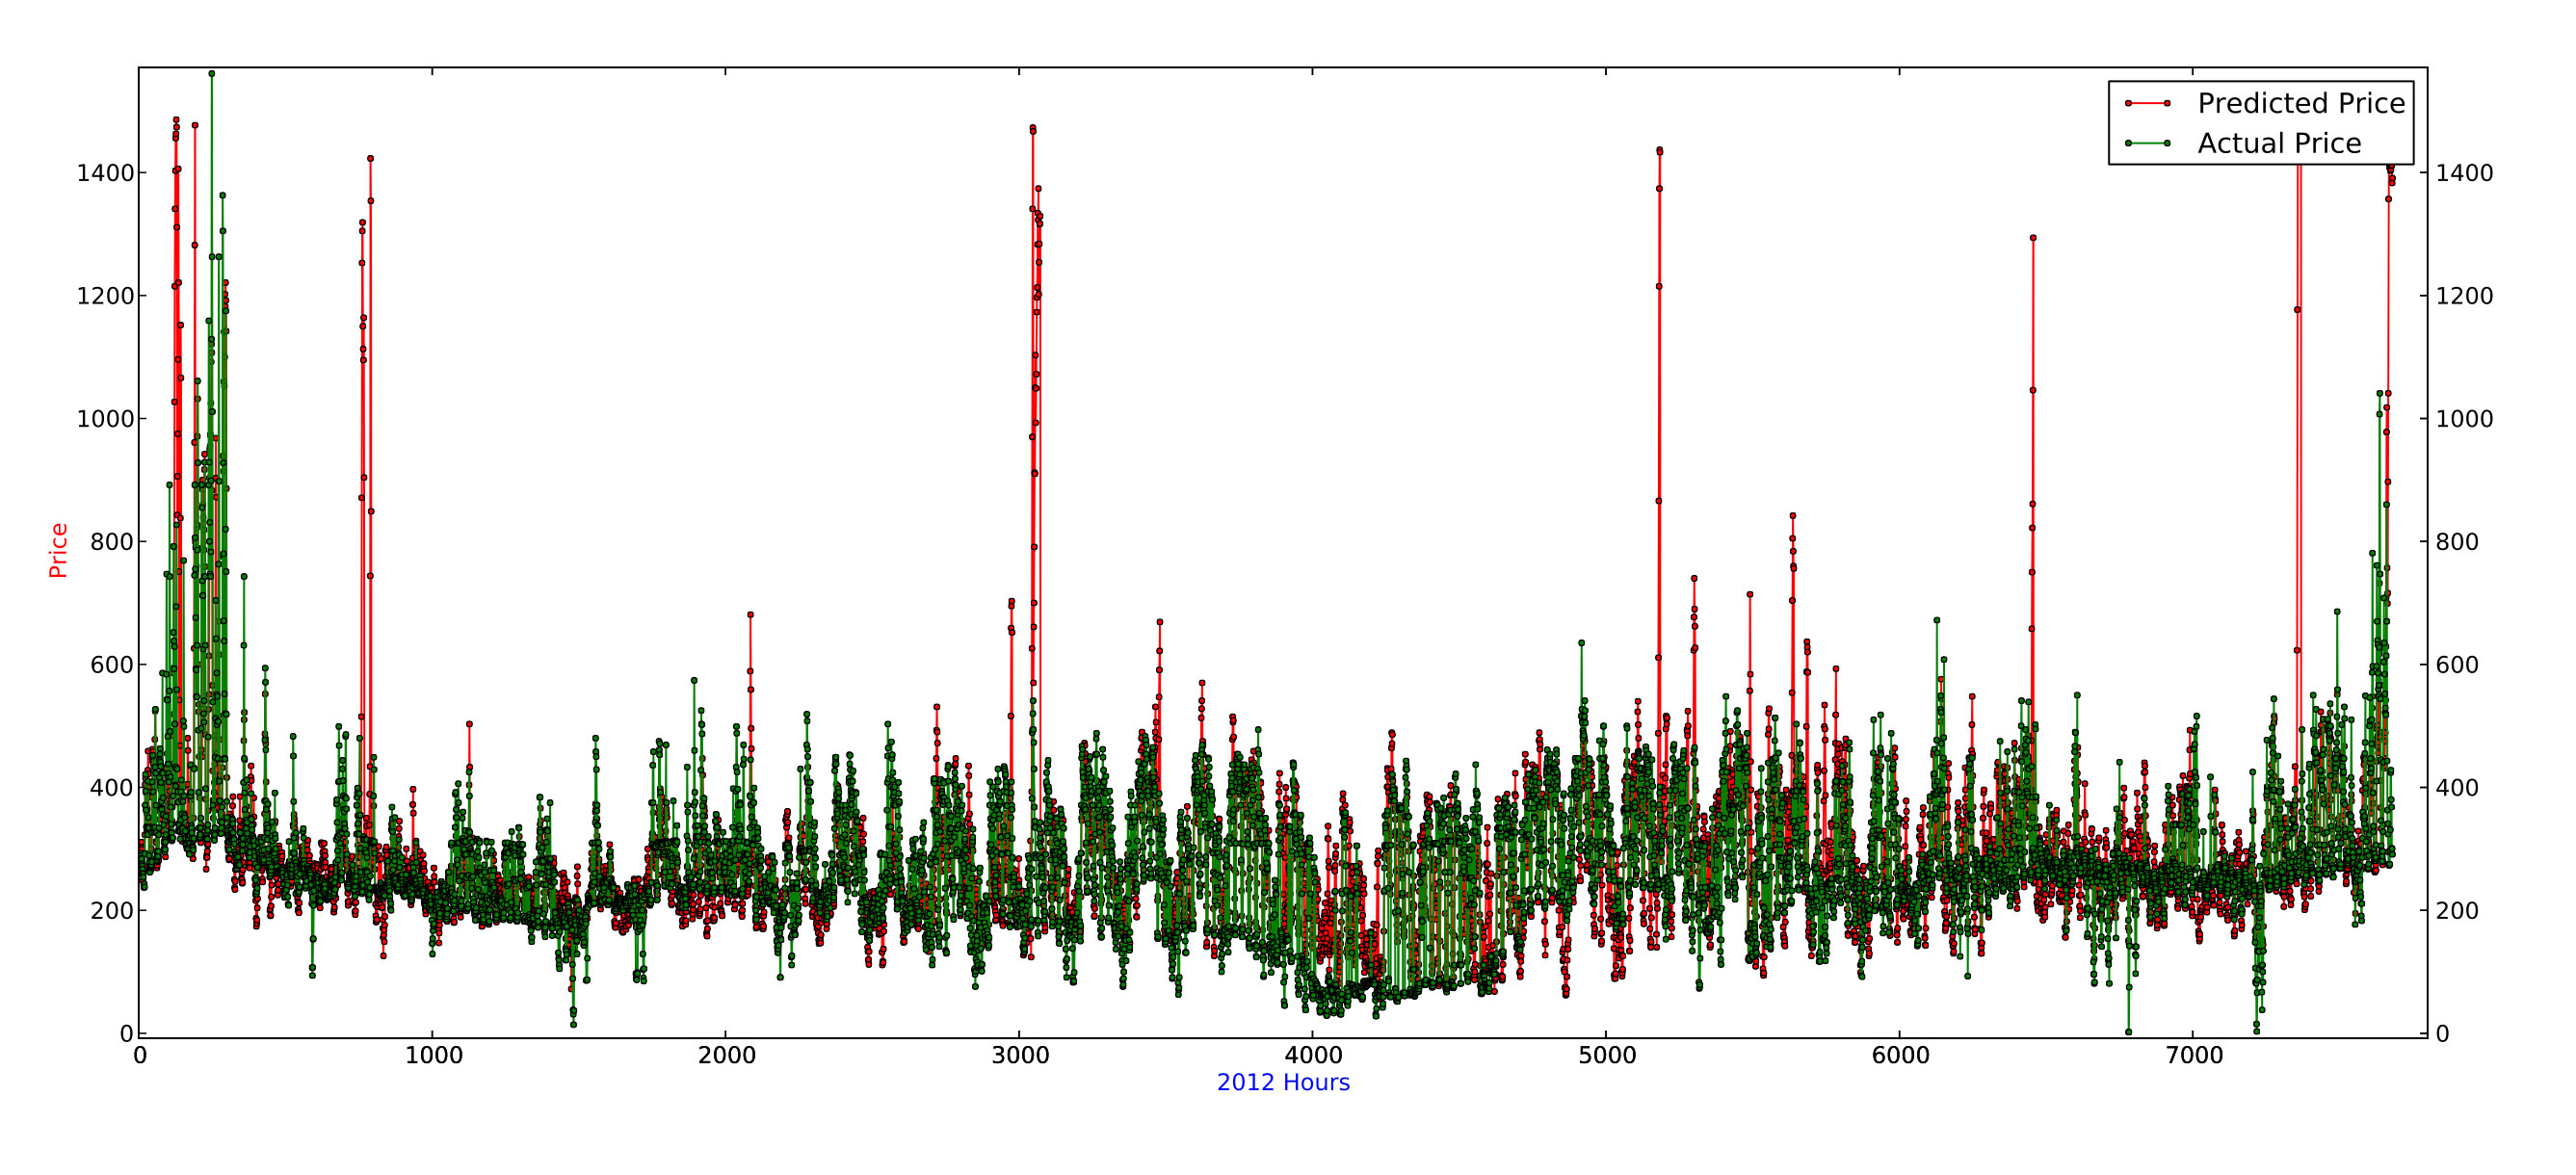
\includegraphics[width=0.85\linewidth,natwidth=898,natheight=587]{billeder/PriceExperimentalAnalysis/NoTrimming.jpg}
\caption{The \#1 forecast with no trimming of the dataset}
\label{fig:NoTrim}
\end{figure}

If we take a look at the same dataset but this time with a 1\% high and low trim (2\% in total) in figure~\ref{fig:1PTrim}; we clearly see that the actual prices in the beginning aren't spiking as heavily as they did in figure~\ref{fig:NoTrim}. This of course prevents us from predicting these high spikes but if we take a look at the rest of the set we see that the 5 faulty spikes have gone as well. This shows the trade off between being able to predict the outliers and the errors they introduce.

\begin{figure}[H]
\centering
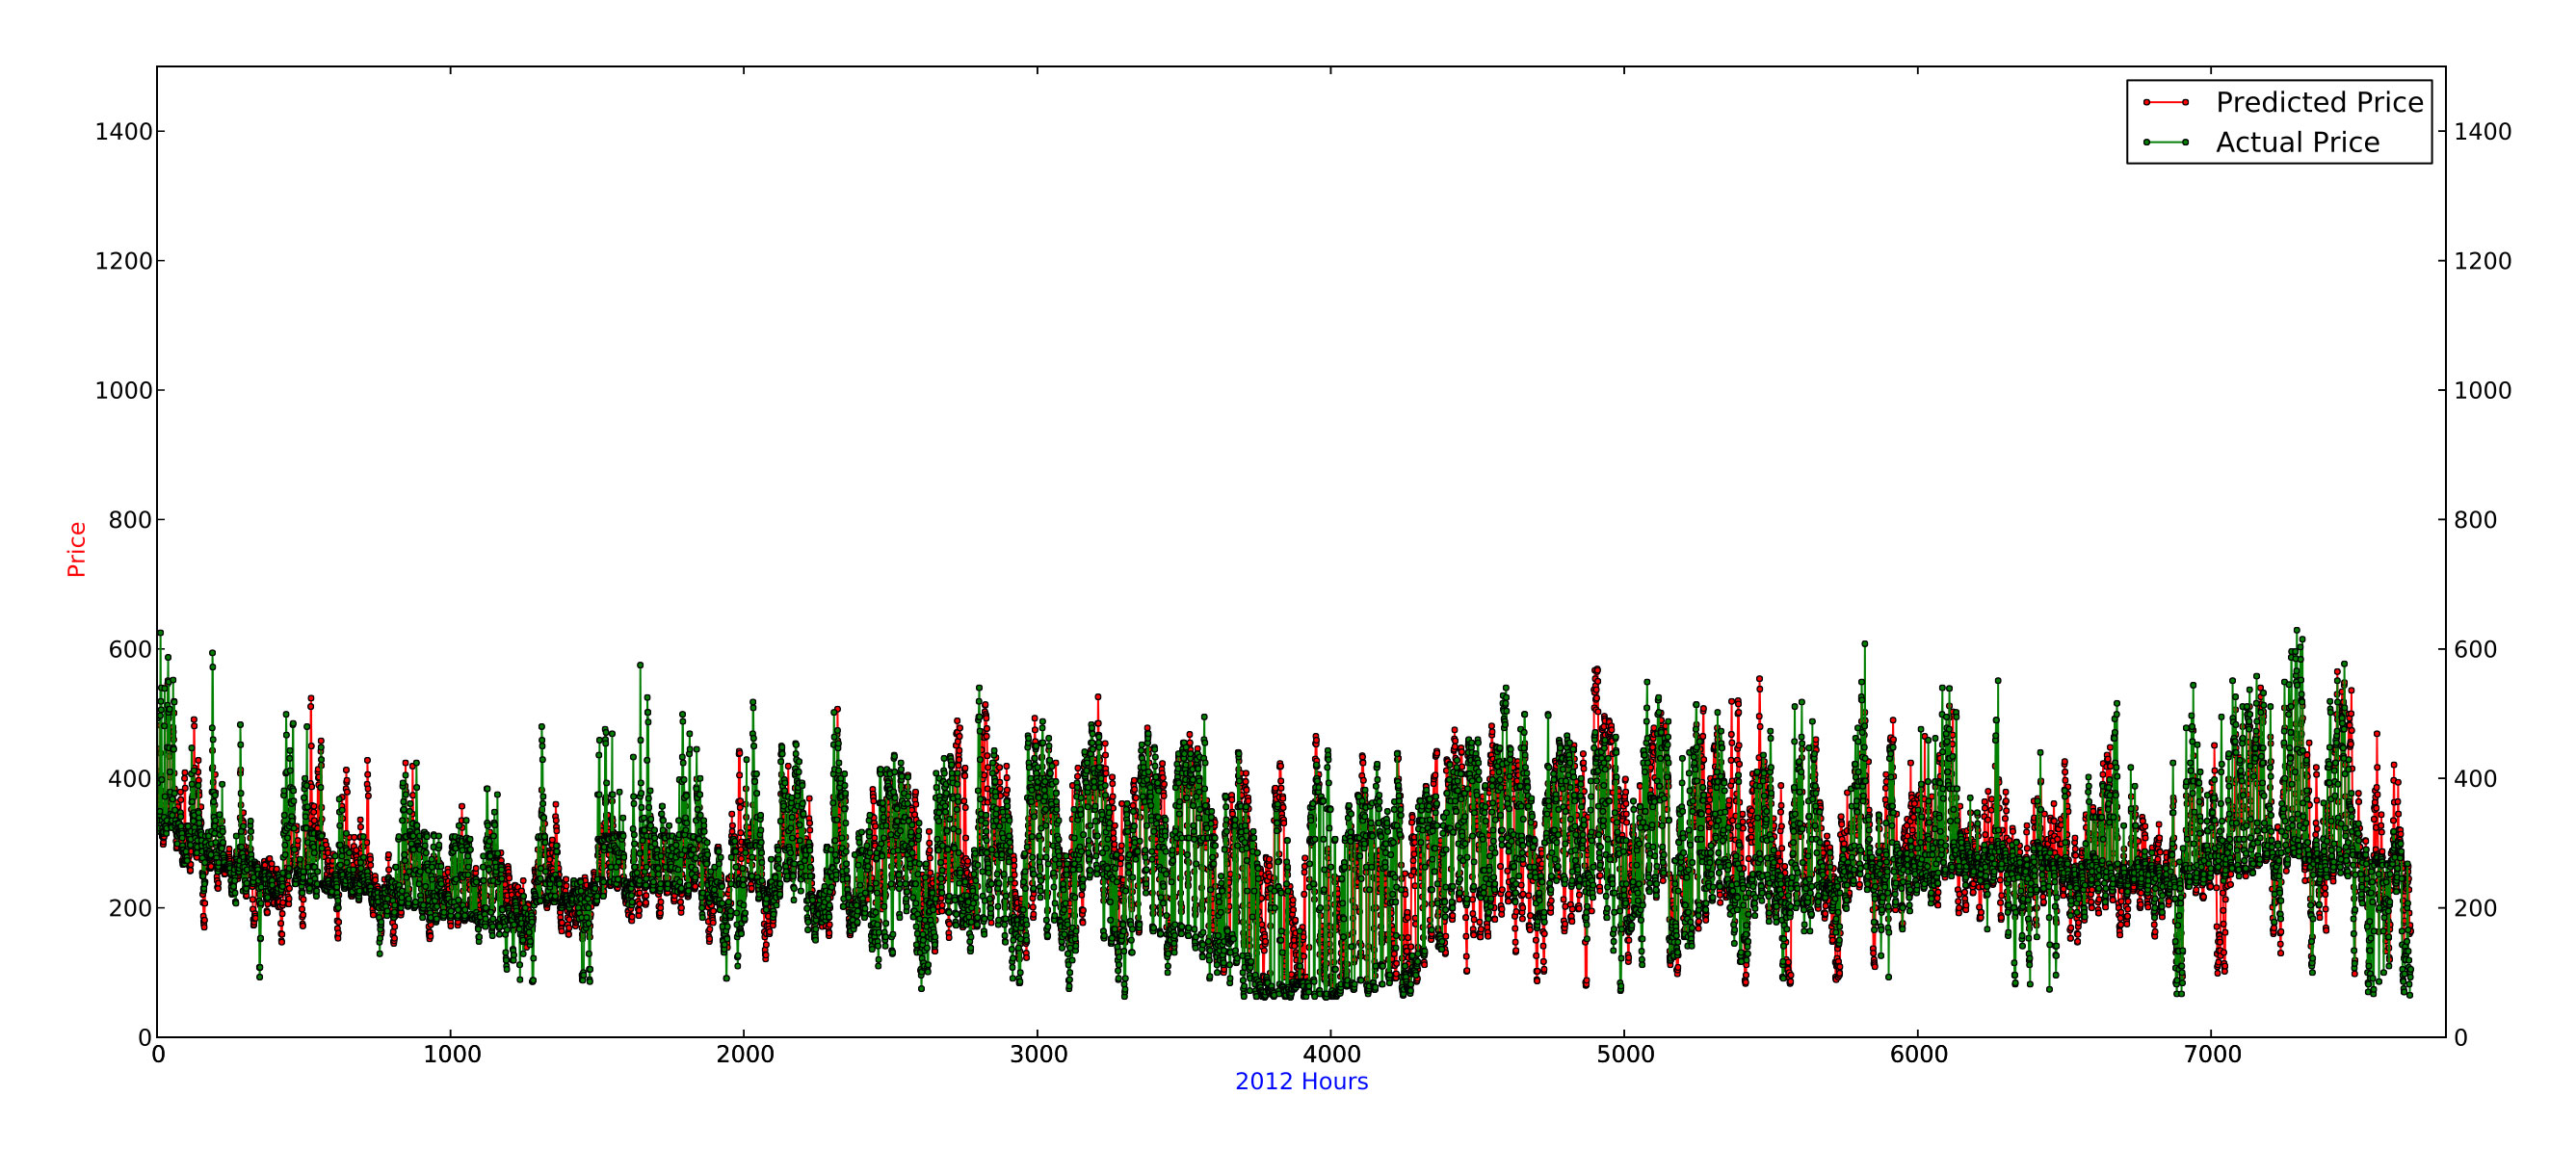
\includegraphics[width=0.85\linewidth,natwidth=898,natheight=587]{billeder/PriceExperimentalAnalysis/1PTrim.jpg}
\caption{The \#1 forecast with 1\% trimming in both ends of the dataset}
\label{fig:1PTrim}
\end{figure}

In figure~\ref{fig:AllTrims} we see the dataset from figure~\ref{fig:1PTrim} with 1\% trim. The lines shows how much would be cut of if we applied 2\%(Purple), 3\%(Red), 4\%(Black) and 5\%(Blue) trimming. Here we clearly see that it is removing data - that is part of the norm - from the set. With every percent we go up we remove 363 entries so at 5\% trim (top and bottom) we will be removing 1815 entries from our dataset. This will result in us never being able to predict value higher or lower than the bars; which we of course are not interested in as most of the values we trim from 2\% and up are part of the standardized dataset.

\begin{figure}[H]
\centering
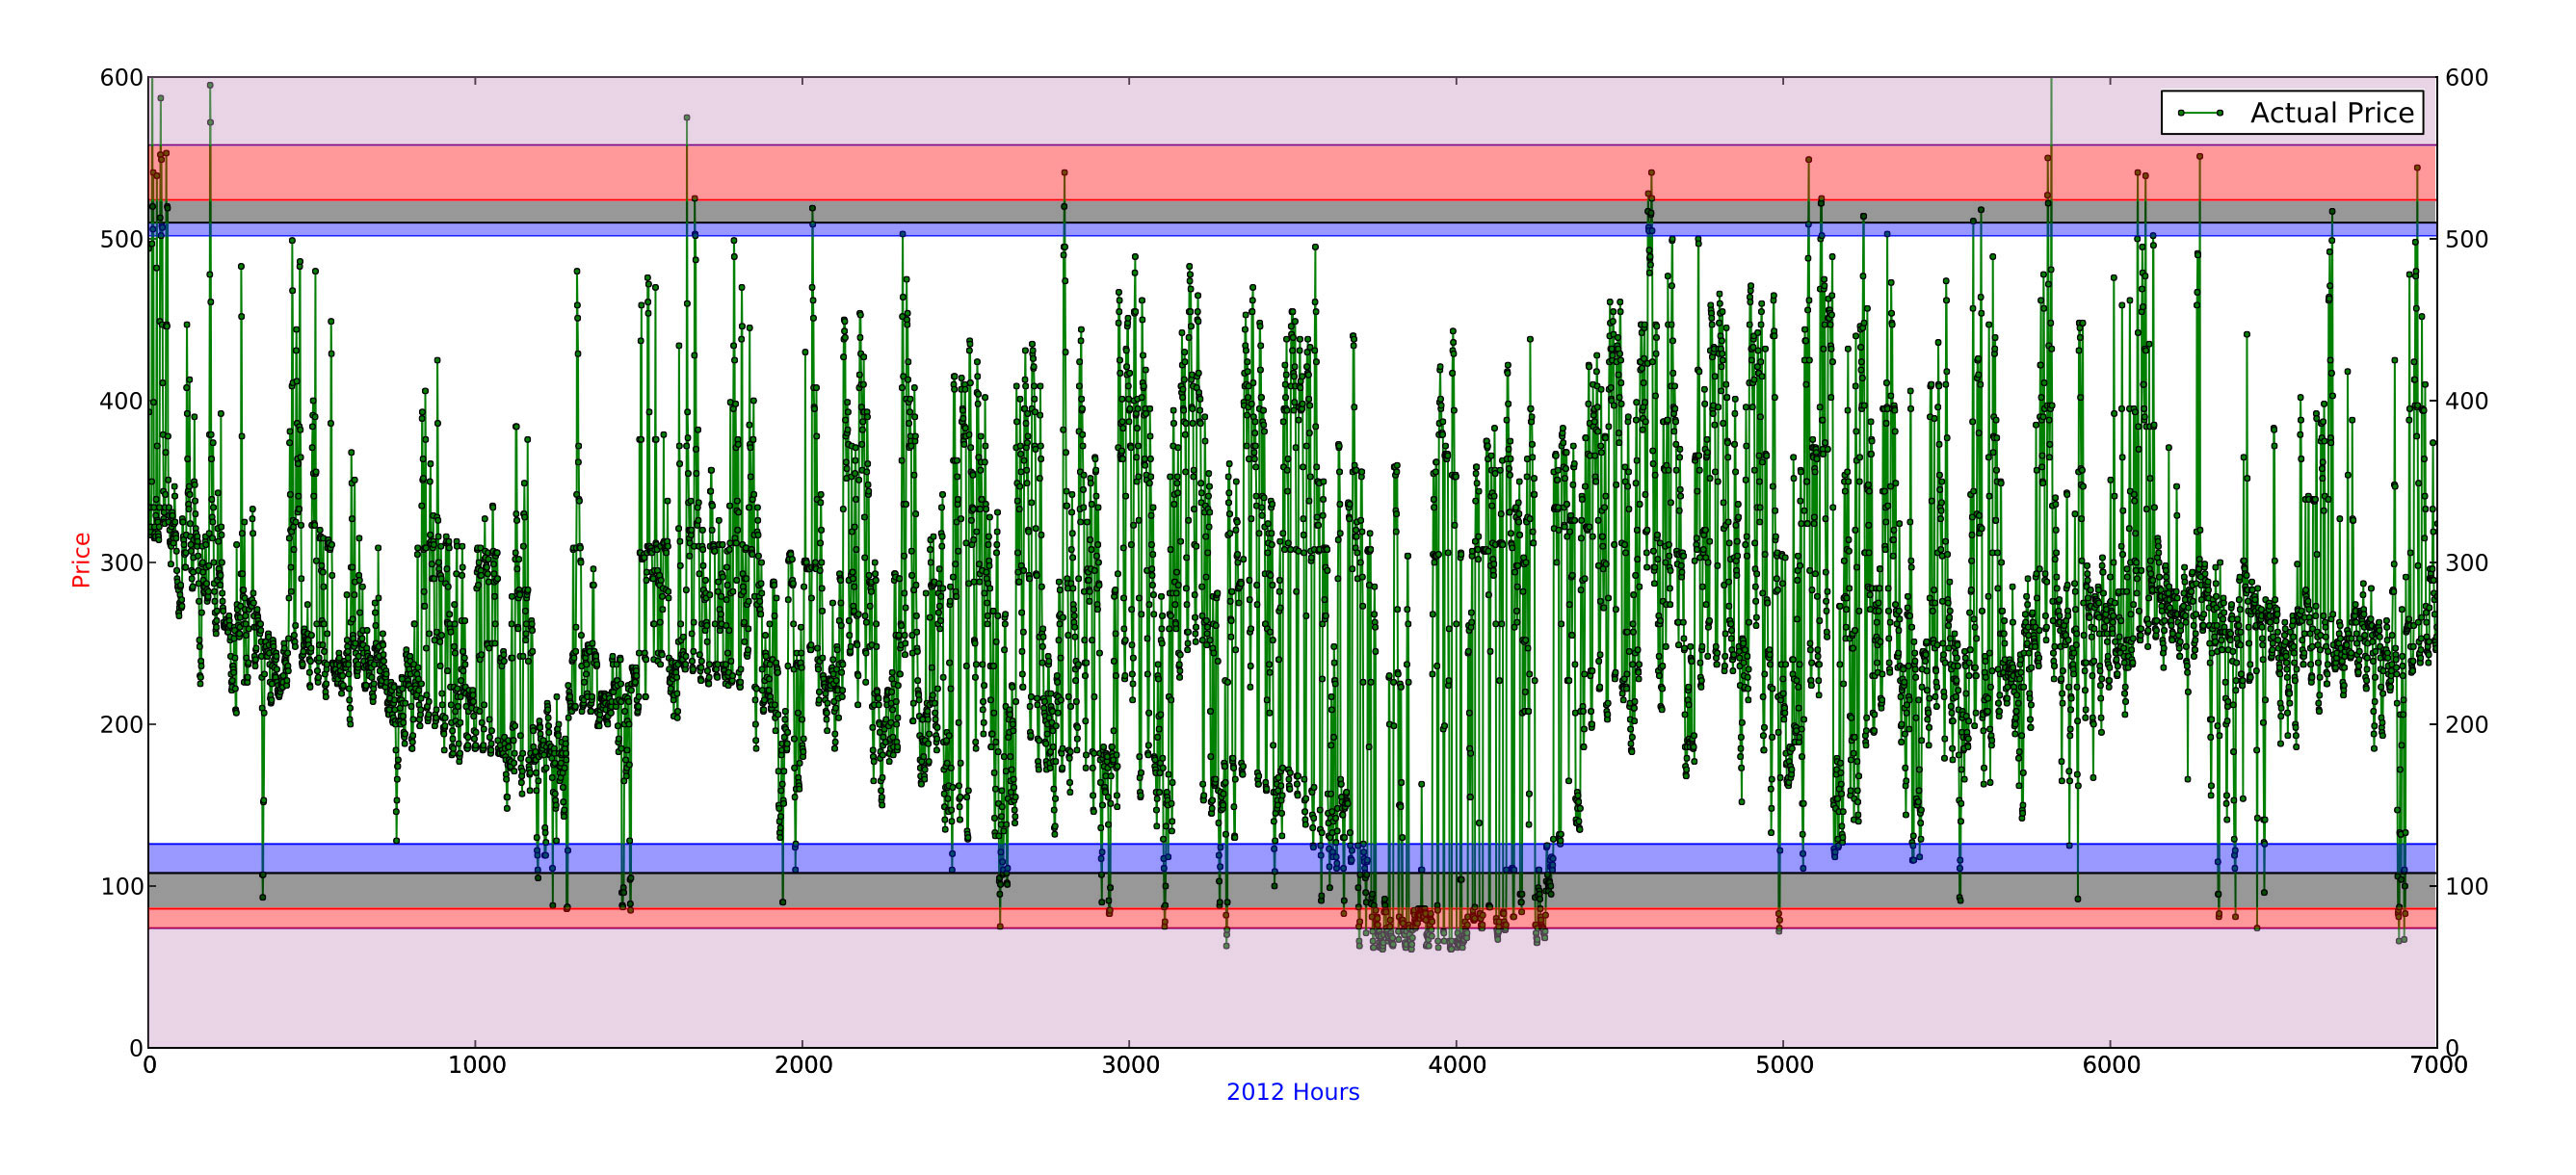
\includegraphics[width=0.85\linewidth,natwidth=898,natheight=587]{billeder/PriceExperimentalAnalysis/restOfTrims.jpg}
\caption{The \#1 forecast with 2\%(Purple), 3\%(Red), 4\%(Black) and 5\%(Blue) trimming in both ends of the dataset}
\label{fig:AllTrims}
\end{figure}

\todo{Skriv om tabellen. Vis sammenhaeng i forhold til 1815 entries vil mistes paa baggrund af en forbedring paa kun 8 MAE i bedste tilfælde.}


\begin{table}[H]
\centering  % used for centering table
\resizebox{0.6\textwidth}{!}{
	\begin{tabular}{|c|c|c|c|c|c|} % centered columns (7 columns)
	\hline
	1PTrim & 2PTrim & 3PTrim & 4PTrim & 5PTrim & Number\\ [0.5ex] % inserts table 
	\hline                  % inserts single horizontal line
	47,21 & 42,90 & 44,48 & 42,46 & 41,79 & \#1 \\ \hline
	46,15 & 43,67 & 43,07 & 39,16 & 40,28 & \#2 \\ \hline
	47,14 & 45,10 & 43,38 & 40,50 & 39,41 & \#3 \\ \hline
	46,70 & 43,96 & 43,21 & 40,03 & 40,29 & \#4 \\ \hline
	45,96 & 43,25 & 45,51 & 40,74 & 40,42 & \#5 \\ \hline
	47,27 & 45,96 & 44,98 & 41,39 & 39,98 & \#6 \\ \hline
	45,93 & 44,66 & 43,39 & 41,02 & 40,40 & \#7 \\ \hline
	46,64 & 42,69 & 44,48 & 41,69 & 40,61 & \#8 \\ \hline
	45,98 & 44,51 & 43,71 & 40,74 & 41,08 & \#9 \\ \hline
	45,60 & 46,07 & 45,81 & 42,52 & 41,32 & \#10 \\ \hline
	\end{tabular}
}
\caption{Trims} % title of Table
\label{table:Top10Trimming} % is used to refer this table in the text
\end{table}

\subsection{Experiment 3: Statistical strategies}

MIXEDPrice ConsumpwindSpeed temperatureRow timeOfDay weekdaysMATRIX monthOfYearMATRIX
\begin{table}[H]
\centering  % used for centering table
\resizebox{0.6\textwidth}{!}{
	\begin{tabular}{|c|c|c|c|c|c|} % centered columns (7 columns)
	\hline
	Curve & Skew & 1Historical & PAPER & MAE & Rank\\ [0.5ex] % inserts table 
	\hline                  % inserts single horizontal line
	       &       & \x    &       & 45.20 & \#1 \\ \hline
	 \x    &       &       &       & 45.58 & \#2 \\ \hline 
	       & \x    & \x    &       & 45.67 & \#3 \\ \hline
	 \x    &       & \x    &       & 46.55 & \#4 \\ \hline
	 \x    & \x    &       &       & 47.03 & \#5 \\ \hline 
	 \x    &       & \x    & \x    & 47.05 & \#6 \\ \hline
	       & \x    & \x    & \x    & 47.48 & \#7 \\ \hline
	       & \x    &       &       & 47.50 & \#8 \\ \hline
	 \x    & \x    & \x    & \x    & 47.72 & \#9 \\ \hline
	       & \x    &       & \x    & 48.03 & \#10 \\ \hline
	       &       & \x    & \x    & 48.09 & \#11 \\ \hline
	 \x    &       &       & \x    & 48.37 & \#12 \\ \hline
	       &       &       & \x    & 48.54 & \#13 \\ \hline
	 \x    & \x    &       & \x    & 49.00 & \#14 \\ \hline
	\end{tabular}
}
\caption{Trims} % title of Table
\label{table:Statistical1} % is used to refer this table in the text
\end{table}

MIXEDPrice Consump windSpeed temperatureRow timeOfDayMATRIX weekdays
\begin{table}[H]
\centering  % used for centering table
\resizebox{0.6\textwidth}{!}{
	\begin{tabular}{|c|c|c|c|c|c|} % centered columns (7 columns)
	\hline
	Curve & Skew & 1Historical & PAPER & MAE & Rank\\ [0.5ex] % inserts table 
	\hline                  % inserts single horizontal line
	 \x    &       &       &       & 43.97 & \#1 \\ \hline
	       &       & \x    &       & 44.38 & \#2 \\ \hline
	       & \x    & \x    &       & 44.60 & \#3 \\ \hline
	       &       & \x    & \x    & 44.96 & \#4 \\ \hline
	 \x    &       & \x    &       & 45.01 & \#5 \\ \hline
	 \x    & \x    & \x    &       & 45.26 & \#6 \\ \hline
	 \x    & \x    &       &       & 45.37 & \#7 \\ \hline
	       &       &       & \x    & 45.67 & \#8 \\ \hline
	 \x    &       & \x    & \x    & 46.46 & \#9 \\ \hline
	       & \x    &       &       & 46.51 & \#10 \\ \hline
	 \x    & \x    & \x    & \x    & 46.52 & \#11 \\ \hline
	 \x    &       &       & \x    & 46.58 & \#12 \\ \hline
	       & \x    &       & \x    & 46.63 & \#13 \\ \hline
	 \x    & \x    &       & \x    & 47.58 & \#14 \\ \hline
	       & \x    & \x    & \x    & 47.80 & \#15 \\ \hline
	\end{tabular}
}
\caption{Trims} % title of Table
\label{table:Statistical2} % is used to refer this table in the text
\end{table}

MIXEDPrice Consump windSpeed temperatureRow timeOfDayMATRIX weekdays monthOfYearMATRIX
\begin{table}[H]
\centering  % used for centering table
\resizebox{0.6\textwidth}{!}{
	\begin{tabular}{|c|c|c|c|c|c|} % centered columns (7 columns)
	\hline
	Curve & Skew & 1Historical & PAPER & MAE & Rank\\ [0.5ex] % inserts table 
	\hline                  % inserts single horizontal line
	       &       & \x    &       & 45.54 & \#1 \\ \hline
	 \x    & \x    & \x    & \x    & 46.12 & \#2 \\ \hline
	 \x    & \x    & \x    &       & 46.34 & \#3 \\ \hline
	       & \x    & \x    &       & 46.40 & \#4 \\ \hline
	       &       &       & \x    & 46.51 & \#5 \\ \hline
	 \x    &       & \x    &       & 46.52 & \#6 \\ \hline
	 \x    & \x    &       &       & 46.57 & \#7 \\ \hline
	 \x    &       &       & \x    & 46.87 & \#8 \\ \hline
	 \x    &       &       &       & 46.93 & \#9 \\ \hline
	       &       & \x    & \x    & 47.03 & \#10 \\ \hline
	       & \x    &       & \x    & 47.15 & \#11 \\ \hline
	       & \x    &       &       & 47.34 & \#12 \\ \hline
	 \x    & \x    &       & \x    & 47.68 & \#13 \\ \hline
	       & \x    & \x    & \x    & 47.87 & \#14 \\ \hline
	\hline %inserts single line
	\end{tabular}
}
\caption{Trims} % title of Table
\label{table:Statistical3} % is used to refer this table in the text
\end{table}

MIXEDPrice Consump windSpeed timeOfDayMATRIX weekdays monthOfYearMATRIX
\begin{table}[H]
\centering  % used for centering table
\resizebox{0.6\textwidth}{!}{
	\begin{tabular}{|c|c|c|c|c|c|} % centered columns (7 columns)
	\hline
	Curve & Skew & 1Historical & PAPER & MAE & Rank\\ [0.5ex] % inserts table 
	\hline                  % inserts single horizontal line
	       &       & \x    &       & 45.87 & \#1 \\ \hline
	       & \x    & \x    &       & 46.68 & \#2 \\ \hline
	       & \x    &       &       & 46.74 & \#3 \\ \hline
	 \x    & \x    & \x    &       & 46.79 & \#4 \\ \hline
	 \x    &       & \x    &       & 47.52 & \#5 \\ \hline
	 \x    &       &       &       & 47.98 & \#6 \\ \hline
	 \x    & \x    &       &       & 48.28 & \#7 \\ \hline
	 \x    &       & \x    &       & 49.18 & \#8 \\ \hline
	       &       & \x    &       & 49.77 & \#9 \\ \hline
	       & \x    & \x    &       & 50.78 & \#10 \\ \hline
	 \x    &       &       &       & 51.44 & \#11 \\ \hline
	 \x    & \x    & \x    &       & 53.93 & \#12 \\ \hline
	       & \x    &       &       & 54.63 & \#13 \\ \hline
	 \x    & \x    &       &       & 55.22 & \#14 \\ \hline
	\end{tabular}
}
\caption{Trims} % title of Table
\label{table:Statistical4} % is used to refer this table in the text
\end{table}

MIXEDPrice Consump windSpeed timeOfDayMATRIX weekdays monthOfYearMATRIX
\begin{table}[H]
\centering  % used for centering table
\resizebox{0.6\textwidth}{!}{
	\begin{tabular}{|c|c|c|c|c|c|} % centered columns (7 columns)
	\hline
	Curve & Skew & 1Historical & PAPER & MAE & Rank\\ [0.5ex] % inserts table 
	\hline                  % inserts single horizontal line
	       & \x    & \x    &       & 45.35 & \#1 \\ \hline
	 \x    & \x    & \x    &       & 45.76 & \#2 \\ \hline
	 \x    &       &       & \x    & 45.83 & \#3 \\ \hline
	 \x    &       &       &       & 46.10 & \#4 \\ \hline
	 \x    & \x    &       &       & 46.40 & \#5 \\ \hline
	 \x    &       & \x    &       & 46.47 & \#6 \\ \hline
	       & \x    &       &       & 46.53 & \#7 \\ \hline
	       &       & \x    & \x    & 46.72 & \#8 \\ \hline
	       &       &       & \x    & 46.88 & \#9 \\ \hline
	 \x    & \x    & \x    & \x    & 47.40 & \#10 \\ \hline
	       & \x    &       & \x    & 47.65 & \#11 \\ \hline
	 \x    &       & \x    & \x    & 47.82 & \#12 \\ \hline
	 \x    & \x    &       & \x    & 47.96 & \#13 \\ \hline
	       & \x    & \x    & \x    & 48.45 & \#14 \\ \hline
	\end{tabular}
}
\caption{Trims} % title of Table
\label{table:Statistical5} % is used to refer this table in the text
\end{table}

MIXEDPrice Consump windSpeed temperatureRow timeOfDayMATRIX weekdays seasonOfYearMATRIX
\begin{table}[H]
\centering  % used for centering table
\resizebox{0.6\textwidth}{!}{
	\begin{tabular}{|c|c|c|c|c|c|} % centered columns (7 columns)
	\hline
	Curve & Skew & 1Historical & PAPER & MAE & Rank\\ [0.5ex] % inserts table 
	\hline                  % inserts single horizontal line
	       & \x    & \x    &       & 45.11 & \#1 \\ \hline
	       &       & \x    &       & 45.24 & \#2 \\ \hline
	 \x    & \x    & \x    &       & 45.43 & \#3 \\ \hline
	 \x    &       &       &       & 45.53 & \#4 \\ \hline
	 \x    & \x    &       & \x    & 46.45 & \#5 \\ \hline
	 \x    & \x    &       &       & 46.56 & \#6 \\ \hline
	       &       & \x    & \x    & 46.76 & \#7 \\ \hline
	 \x    &       & \x    &       & 46.87 & \#8 \\ \hline
	       & \x    & \x    & \x    & 47.25 & \#9 \\ \hline
	       & \x    &       &       & 47.88 & \#10 \\ \hline
	 \x    & \x    & \x    & \x    & 48.01 & \#11 \\ \hline
	 \x    &       & \x    & \x    & 48.13 & \#12 \\ \hline
	       & \x    &       & \x    & 48.40 & \#13 \\ \hline
	 \x    &       &       & \x    & 49.68 & \#14 \\ \hline
	\end{tabular}
}
\caption{Trims} % title of Table
\label{table:Statistical6} % is used to refer this table in the text
\end{table}

MIXEDPrice Consump windSpeed temperatureRow timeOfDayMATRIX monthOfYearMATRIX
\begin{table}[H]
\centering  % used for centering table
\resizebox{0.6\textwidth}{!}{
	\begin{tabular}{|c|c|c|c|c|c|} % centered columns (7 columns)
	\hline
	Curve & Skew & 1Historical & PAPER & MAE & Rank\\ [0.5ex] % inserts table 
	\hline                  % inserts single horizontal line
	       &       & \x    & \x    & 45.14 & \#1 \\ \hline
	       &       &       & \x    & 45.55 & \#2 \\ \hline
	       & \x    &       &       & 45.56 & \#3 \\ \hline
	       & \x    &       & \x    & 45.60 & \#4 \\ \hline
	 \x    &       & \x    &       & 45.91 & \#5 \\ \hline
	 \x    & \x    & \x    & \x    & 45.95 & \#6 \\ \hline
	 \x    & \x    &       &       & 45.99 & \#7 \\ \hline
	 \x    &       &       & \x    & 46.14 & \#8 \\ \hline
	 \x    &       &       &       & 46.58 & \#9 \\ \hline
	 \x    & \x    &       & \x    & 46.87 & \#10 \\ \hline
	       &       & \x    &       & 46.98 & \#11 \\ \hline
	       & \x    & \x    & \x    & 47.02 & \#12 \\ \hline
	 \x    & \x    & \x    &       & 47.08 & \#13 \\ \hline
	 \x    &       & \x    & \x    & 47.94 & \#14 \\ \hline
	       & \x    & \x    &       & 47.98 & \#15 \\ \hline
	\end{tabular}
}
\caption{Trims} % title of Table
\label{table:Statistical7} % is used to refer this table in the text
\end{table}

MIXEDPrice Consump windSpeed temperatureRow timeOfDayMATRIX seasonOfYearMATRIX
\begin{table}[H]
\centering  % used for centering table
\resizebox{0.6\textwidth}{!}{
	\begin{tabular}{|c|c|c|c|c|c|} % centered columns (7 columns)
	\hline
	Curve & Skew & 1Historical & PAPER & MAE & Rank\\ [0.5ex] % inserts table 
	\hline                  % inserts single horizontal line
	       &       & \x    &       & 44.72 & \#1 \\ \hline
	       & \x    &       &       & 45.23 & \#2 \\ \hline
	       & \x    &       & \x    & 45.95 & \#3 \\ \hline
	 \x    & \x    & \x    &       & 46.02 & \#4 \\ \hline
	       & \x    & \x    &       & 46.04 & \#5 \\ \hline
	 \x    & \x    &       & \x    & 46.09 & \#6 \\ \hline
	 \x    &       & \x    & \x    & 46.43 & \#7 \\ \hline
	 \x    & \x    &       &       & 46.45 & \#8 \\ \hline
	 \x    &       & \x    &       & 46.47 & \#9 \\ \hline
	 \x    & \x    & \x    & \x    & 46.50 & \#10 \\ \hline
	       & \x    & \x    & \x    & 46.62 & \#11 \\ \hline
	       &       & \x    & \x    & 47.06 & \#12 \\ \hline
	 \x    &       &       & \x    & 47.26 & \#13 \\ \hline
	       &       &       & \x    & 47.41 & \#14 \\ \hline
	 \x    &       &       &       & 47.89 & \#15 \\ \hline
	\end{tabular}
}
\caption{Trims} % title of Table
\label{table:Statistical8} % is used to refer this table in the text
\end{table}

MIXEDPrice Consump windSpeed temperatureRow timeOfDay weekdays seasonOfYearMATRIX
\begin{table}[H]
\centering  % used for centering table
\resizebox{0.6\textwidth}{!}{
	\begin{tabular}{|c|c|c|c|c|c|} % centered columns (7 columns)
	\hline
	Curve & Skew & 1Historical & PAPER & MAE & Rank\\ [0.5ex] % inserts table 
	\hline                  % inserts single horizontal line
       & \x    & \x    &       & 45.58 & \#1 \\ \hline
       &       & \x    &       & 46.22 & \#2 \\ \hline
 \x    &       & \x    &       & 46.36 & \#3 \\ \hline
       &       & \x    & \x    & 46.75 & \#4 \\ \hline
 \x    & \x    &       & \x    & 46.81 & \#5 \\ \hline
 \x    & \x    &       &       & 46.97 & \#6 \\ \hline
 \x    & \x    & \x    &       & 47.04 & \#7 \\ \hline
       & \x    &       & \x    & 47.22 & \#8 \\ \hline
       & \x    &       &       & 47.26 & \#9 \\ \hline
 \x    &       &       & \x    & 47.32 & \#10 \\ \hline
 \x    &       &       &       & 47.47 & \#11 \\ \hline
       &       &       & \x    & 47.64 & \#12 \\ \hline
       & \x    & \x    & \x    & 47.76 & \#13 \\ \hline
 \x    &       & \x    & \x    & 48.48 & \#14 \\ \hline
 \x    & \x    & \x    & \x    & 48.73 & \#15 \\ \hline
	\end{tabular}
}
\caption{Trims} % title of Table
\label{table:Statistical9} % is used to refer this table in the text
\end{table}

MATRIX Price Consump windSpeed timeOfDay weekdays monthOfYear
\begin{table}[H]
\centering  % used for centering table
\resizebox{0.6\textwidth}{!}{
	\begin{tabular}{|c|c|c|c|c|c|} % centered columns (7 columns)
	\hline
	Curve & Skew & 1Historical & PAPER & MAE & Rank\\ [0.5ex] % inserts table 
	\hline                  % inserts single horizontal line
	       & \x    & \x    &       & 45.20 & \#1 \\ \hline
	       &       &       & \x    & 46.78 & \#2 \\ \hline
	 \x    &       &       &       & 46.83 & \#3 \\ \hline
	       & \x    &       &       & 47.00 & \#4 \\ \hline
	       &       & \x    &       & 47.06 & \#5 \\ \hline
	 \x    &       & \x    & \x    & 47.13 & \#6 \\ \hline
	 \x    & \x    & \x    &       & 47.36 & \#7 \\ \hline
	       &       & \x    & \x    & 47.51 & \#8 \\ \hline
	 \x    & \x    &       &       & 47.99 & \#9 \\ \hline
	 \x    & \x    &       & \x    & 48.30 & \#10 \\ \hline
	 \x    &       &       & \x    & 48.56 & \#11 \\ \hline
	 \x    & \x    & \x    & \x    & 48.63 & \#12 \\ \hline
	       & \x    &       & \x    & 48.77 & \#13 \\ \hline
	\end{tabular}
}
\caption{Trims} % title of Table
\label{table:Statistical10} % is used to refer this table in the text
\end{table}

\subsubsection{Experiment 4: Black box optimization}

